\section{Methodology}\label{methodology}

The main goal of our research is to produce a complete, correct taxonomy of
software testing terminology. However, we cannot do this without understanding
its current state. Therefore, we start by documenting how the literature
currently uses testing terminology, both correctly and incorrectly. This
results in a big messy glossary of software testing terms, along with a list of
flaws. Once we analyze these data, including how and why these flaws emerge, we
can start to resolve them. For now, we document the current (messy) state of
software testing terminology by:

\input{build/methodOverview}

\subsection{Sources}\label{sources}
As there is no single authoritative source on software testing terminology,
we need to look at many sources to observe how this terminology is used in
practice. Since we are particularly interested in software engineering, we
start from the vocabulary document for systems and software engineering%
\qtodo{Better name for this?}
\citep{IEEE2017} and two versions of the \acf{swebok}---the newest
one \citep{SWEBOK2014} and one submitted for public review\footnote{
    \refHelper \citep{SWEBOK2024} has been published since we investigated
    these sources; if time permits, we will revisit this published version.
} \citep{SWEBOK2024}. To gather further sources, we then use a version of
``snowball sampling'',
which ``is commonly used to locate hidden populations \dots{} [via] referrals
from initially sampled respondents to other persons'' \citep{Johnson2014}. We
apply this concept to ``referrals'' between sources. \addTextEx{} We similarly
``snowball'' on terminology itself; when a term requires more investigation
(e.g., its definition is missing or unclear), we perform a
miniature literature review on this subset to ``fill in'' this missing
information (see \Cref{undef-terms}). We may then investigate these additional
sources in their entirety, as opposed to just the original subset of interest,
based on our heuristic of credibility (defined in \Cref{cred}) and how much
extra information they provide.

For ease of discussion and analysis, we group the complete set of sources into
``tiers'' based on their format, method of publication, and credibility. We
therefore create the following tiers, given in order of descending credibility:
\begin{enumerate}
    \item established standards (\Cref{stds}),
    \item terminology collections (\Cref{metas}),
    \item textbooks (\Cref{texts}), and
    \item papers and other documents (\Cref{papers}).
\end{enumerate}
A summary of how many sources comprise each tier is given in
\Cref{fig:sourceSummary}\ifnotpaper; complete lists of sources for each tier
are given in \Cref{app-src-tiers}\fi. We often use papers to ``fill in'' missing
information in a more specific subdomain and do not always investigate them
entirely (see \Cref{undef-terms}), which results in a large number of them. We
use standards the second most frequently due to their high credibility and
broad scope; for example, the glossary portion of \citet{IEEE2017} has 514
pages! Using these standards allows us to record many test approaches in a
similar context from a source that is widely used and well-respected.

% Only top or bottom to comply with IEEE guidelines
\begin{figure}[bt!]
    \centering
    \begin{tikzpicture}
        \pie[sum=auto, after number=, text=legend, thick,
            scale=\ifnotpaper0.7\else0.5\fi,
            every label/.style={align=left, scale=0.7}]
        {\stdSources{3}/\stds{},
            \metaSources{3}/\metas{},
            \textSources{3}/\texts{},
            \paperSources{3}/\papers{}}
    \end{tikzpicture}
    \caption{Summary of how many sources comprise each source tier.}
    \label{fig:sourceSummary}
\end{figure}

\subsubsection{\stdSources{1}}
\label{stds}
% Colored \textcolor{green}{green}

These are documents written for the field of software engineering by reputable
standards bodies, namely ISO, the \acf{iec}, and IEEE. Their purpose is to
``encourage the use of systems and software engineering standards'' and
``collect and standardize terminology'' by ``provid[ing] definitions that are
rigorous, uncomplicated, and understandable by all concerned''
\citep[p.~viii]{IEEE2017}. For these reasons, they
are the most credible sources. However, this does not imply perfection, as we
identify \stdFlawDmnBrkdwn{13} % is (should be!) equal to \stdFlawMnfstBrkdwn{13}
flaws within these standards (see \Cref{tab:flawMnfsts,tab:flawDmns})!
Only standards for software development and testing are in scope for
this research (see \Cref{scope}). For example, ``the purpose of the
ISO/IEC/IEEE 29119 series is to define an internationally agreed set of
standards for software testing that can be used by any organization when
performing any form of software testing''
\ifnotpaper(\fi\citeyear[p.~vii]{IEEE2022}\ifnotpaper; similar in
\citeyear[p.~ix]{IEEE2016})\fi.

\subsubsection{\metaSources{1}}
\label{metas}
% Colored \textcolor{blue}{blue}

These are collections of software testing terminology built up from multiple
sources, such as the established standards outlined in \Cref{stds}. For
example, the \acs{swebok} is ``proposed as a
suitable foundation for government licensing, for the regulation of software
engineers, and for the development of university curricula in software
engineering'' \citep[p.~xix]{KanerEtAl2011}. Even though it is ``published by
the IEEE Computer Society'', it ``reflects the current state of generally
accepted, consensus-driven knowledge derived from the interaction between
software engineering theory and practice'' \citep{AboutSWEBOK}. Due to this
combination of IEEE standards and state-of-the-practice observations, we
designate it as a collection of terminology as opposed to an established
standard. Collections such as this are often written by a large
organization, such as the \acf{istqb}, but not always. \ifnotpaper \else
    \citeauthor{Firesmith2015} \fi \citet{Firesmith2015}'s taxonomy presents
relations between many test approaches and \ifnotpaper \else
    \citeauthor{DoğanEtAl2014} \fi \citet{DoğanEtAl2014}'s literature
review cites many sources from which we can ``snowball'' if desired
(see \Cref{sources}), so we include them in this tier as well.

\subsubsection{\textSources{1}}
\label{texts}
% Colored \textcolor{Maroon}{maroon}

We consider textbooks to be more credible than papers (see \Cref{papers})
because they are widely used as resources for teaching software engineering and
industry frequently uses them as guides. Although textbooks have smaller sets of
authors, they follow a formal review process before publication. Textbooks used
at McMaster University \citep{Patton2006,PetersAndPedrycz2000,vanVliet2000}
served as the original (albeit ad hoc and arbitrary) starting point of this
research, and we investigate other books as they arise. \addTextEx{}

\subsubsection{\paperSources{1}}
\label{papers}
% Colored black

The remaining documents all have much smaller sets of authors and are much less
widespread than those in higher source tiers. While most of these are journal
articles and conference papers, we also include the following document types.
Some of these are not peer-reviewed works but are still useful for
observing how terms are used in practice\thesisissueref{89}:

\begin{itemize}
    \item Report \citep{Kam2008,Gerrard2000a,Gerrard2000b}
    \item Thesis \citep{Bas2024}
          % \item A less-formal classification \citep{KuļešovsEtAl2013}
    \item Website \citep{LambdaTest2024,Pandey2023}
    \item Booklet \citep{SPICE2022}
    \item \ifnotpaper \else ChatGPT \fi \citet{ChatGPT2024} (with its claims
          supported by \citet{RusEtAl2008})
\end{itemize}

% Moved here to display nicely in paper
\ifnotpaper\else
    % Only top or bottom to comply with IEEE guidelines
    \begin{table*}[t!]
        \ieeeCatsTable{}
    \end{table*}
\fi

\subsection{Procedure}\label{procedure}

We track terminology used in the literature by building glossaries. The one
most central to our research is \ourApproachGlossary{}, where we give each
test approach its own row to record its name and any given \approachFields{}.
If no category is given, the ``approach'' category is assigned
(with no accompanying citation) as a ``catch-all'' category. All other fields
may be left blank, but a lack of definition indicates that the approach should
be investigated further to see if its inclusion is meaningful (see
\Cref{undef-terms}). Any additional information from other sources is added to
or merged with the existing information in our glossary where appropriate.
This includes the generic ``approach'' category being replaced with a more
specific one, an additional synonym being mentioned, or another source
describing an already-documented parent-child relation. If any new information
does not agree with existing information or indicates a potential flaw, we
record it in our glossary as dubious information (see \Cref{imp-case-four})
or in a separate document if it is clearly flawed (see \Cref{flaw-def}).
When new information does not conflict with existing information, we either
keep the clearest and most concise version or merge them to paint a more
complete picture. Finally, we record any other notes, such as questions,
prerequisites, and other resources to investigate.

For example, \citet[p.~1, 36]{IEEE2022} \multiAuthHelper{define} ``A/B testing''
(see \Cref{fig:IEEE-A-B-Testing}), giving ``split-run testing'' as a synonym
and describing it as ``statistical testing approach''. We therefore create a
new row in \ourApproachGlossary{} for ``A/B Testing'' with the
Category\qtodo{Should glossary headers be capitalized?}
of ``Approach'', a Synonym of ``Split-Run Testing'', and a
Parent of ``Statistical Testing'' (based on \Cref{par-chd-rels}), all with
their relevant citations. We then abstract away this already-captured
information from its Definition before recording it as ``testing `that allows
testers to determine which of two systems or components performs better'\,''
with the same citation information \citep[pp.~1, 36]{IEEE2022}. The latter page
provides more information that we capture as Notes in our glossary: it ``can be
time-consuming, although tools can be used to support it'', ``is a means of
solving the test oracle problem by using the existing system as a partial
oracle'', and is ``not a test case generation technique as test inputs are not
generated'' \citetext{p.~36}. Interestingly, this explicitly rules out
``Technique'' as a possible Category for this approach, which is consistent
with its categorization as a test practice \citetext{Fig.~2}; we replace our
previous Category of ``Approach'' with the more specific ``Practice''
(see \Cref{cats-def}).
\begin{figure}[bt!]
    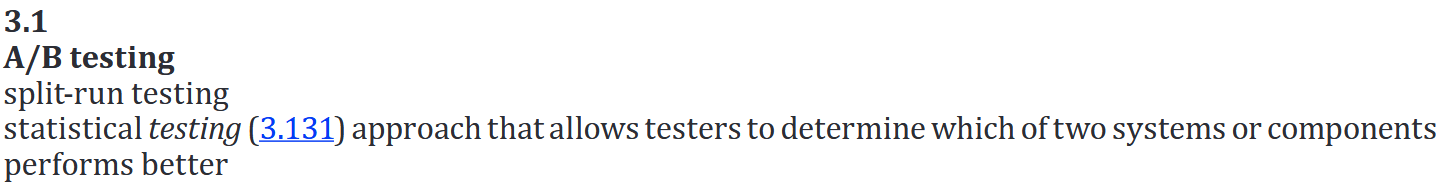
\includegraphics[width=\linewidth]{assets/images/a-b testing.png}
    \caption{\refHelper \citet[p.~1]{IEEE2022}'s glossary entry for
        ``A/B testing''.}\label{fig:IEEE-A-B-Testing}
\end{figure}
As we investigate other sources, we learn more about this approach. \refHelper
\citet[p.~58]{Firesmith2015} gives it as a child of usability testing, so we
include this Parent alongside ``Statistical Testing'' without issue. However,
since usability testing is a test type \ifnotpaper
    (\citealp[pp.~22, 26\=/27]{IEEE2022}; \citeyear[pp.~7, 40, Tab.~A.1]{IEEE2021};
    implied by its quality; \citealp[p.~53]{Firesmith2015})\else
    \cite[pp.~22, 26\=/27]{IEEE2022}, \cite[pp.~7, 40, Tab.~A.1]{IEEE2021}\fi,
A/B testing may inherit this categorization. We document this by adding
``Type'' as a Category alongside ``Practice'' with the source ``inferred from
usability testing''. Since this violates our assumption that categories are
orthogonal\ifnotpaper\ (see \Cref{orth-approach})\fi, we consider this to be
an inferred flaw\ifnotpaper, defined in \Cref{infers} and documented later in
\Cref{auto-flaw-analysis,tab:infMultiCats}\else\ (details omitted for brevity)\fi.

We use similar procedures to track software qualities \ifnotpaper (see
    \Cref{qual-test}) \fi and supplementary terminology (either shared by
multiple approaches or too complicated to explain inline) in separate
glossaries with a similar format. This includes recording the name, definition,
and synonym(s) of these terms, as well as any precedence for a related test
type for a given software quality. For example, analyzability\footnote{
    This may be spelled ``analyzability'' \citep[p.~18]{IEEE2017} or
    ``analysability'' \citep{ISO_IEC2023a}; since this is a dialectal
    difference, we do not count this as a label flaw (see
    \Cref{label-flaw-def}).}, modifiability, modularity, reusability, and
testability are all subqualities of maintainability \ifnotpaper
    (\citealp{ISO_IEC2023a}; \citealp[Tab.~A.1]{IEEE2021};
    \citealp[p.~7\=/10]{SWEBOK2024}) \else
    \cite[p.~7\=/10]{SWEBOK2024}, \cite[Tab.~A.1]{IEEE2021},
    \cite{ISO_IEC2023a} \fi which has an associated test type
\ifnotpaper
    (\citealp[pp.~5, 22]{IEEE2022}; \citeyear[p.~38, Tab.~A.1]{IEEE2021})\else
    \cite[pp.~5, 22]{IEEE2022}, \cite[p.~38, Tab.~A.1]{IEEE2021}\fi. This sets
a ``precedent'' for each of these subqualities having its own associated test
type (e.g., reusability testing). \ifnotpaper
    Sometimes, the literature provides a relation between qualities where at
    least one of them does not have an explicit approach associated with it
    (although it may be derived; see \Cref{cov-test}). For example,
    \citet{ISO_IEC2023a} provides relations involving dependability and
    modifiability; since only the qualities are described, we do not record
    their implicit related approaches and omit these relations when generating
    graphs as described in \Cref{graph-gen}.\fi

We use heuristics to guide this process for all three
glossaries to increase confidence that all terms are identified, paying
special attention to the following when investigating a new source:
\begin{itemize}
    \item glossaries, taxonomies, hierarchies, and lists of terms,
    \item testing-related terms (e.g., terms containing ``test(ing)'',
          \ifnotpaper ``review(s)'', ``audit(s)'', \fi
          ``validation'', or ``verification''),
    \item terms that had emerged as part of already-discovered
          testing approaches, \emph{especially} those that were ambiguous
          or prompted further discussion (e.g., terms containing
          ``performance'', ``recovery'', ``component'', ``bottom-up'',
          \ifnotpaper ``boundary'', \fi or ``configuration''), and
    \item terms that imply test approaches\ifnotpaper\footnote{
                  Since these methods for deriving test approaches only arose
                  as research progressed, some examples would have been missed
                  during the first pass(es) of resources investigated earlier
                  in the process. While reiterating over them would be ideal,
                  this may not be possible due to time constraints.
              } (see \Cref{derived-tests})\fi.
\end{itemize}
We apply these heuristics to most investigated sources, especially established
standards (see \Cref{stds}), in their entirety. Some sources, however, we only
partially investigate, such as those chosen for a specific area of
interest or based on a test approach that was determined to be out-of-scope.
These include the following sources as described in \Cref{undef-terms}:
\citet{ISO2022,ISO2015,Dominguez-PumarEtAl2020,PierreEtAl2017,
    TrudnowskiEtAl2017,YuEtAl2011,Tsui2007,Goralski1999}.
During the first pass of data collection, we investigate and record all
terminology related to software testing. Some of these terms are less
applicable to our original motivation of test case automation \ifnotpaper
    (such as static testing; see \Cref{static-test}\thesisissueref{39}) \fi or
are quite broad\ifnotpaper\ (such as attacks; see
    \Cref{attacks}\thesisissueref{55})\fi, so we will omit them during future
analysis.

\subsubsection{Derived Test Approaches}\label{derived-tests}

Throughout this research, we noticed many groups of test approaches that arise
from some underlying area of software (testing) knowledge. The legitimacy of
extrapolating new test approaches from these knowledge domains is heavily
implied by the literature, but not explicitly stated as a general rule. Regardless,
since the field of software is ever-evolving, it is crucial to be able to
adapt to, talk about, and understand new developments in software testing.
Bases for defining new test approaches suggested by the literature include
coverage metrics, software qualities, and attacks. These are meaningful
enough to merit analysis and are therefore in scope. Requirements may also
imply related test approaches, but this mainly results in test approaches
that would be out of scope. Other test approaches found in the literature
are derived from programming languages or other orthogonal test approaches,
but these are out of scope as this information is better captured by other
approaches.

\ifnotpaper
    \paragraph{Coverage-driven Techniques}\label{cov-test}

    Test techniques are able to ``identify test coverage items \dots{} and
    derive corresponding test cases''
    \ifnotpaper
        (\citealp[p.~11]{IEEE2022}; similar in \citeyear[p.~467]{IEEE2017})
    \else
        \cite[p.~11]{IEEE2022} (similar in \cite[p.~467]{IEEE2017})
    \fi
    in a ``systematic'' way
    \citeyearpar[p.~464]{IEEE2017}.
    \ifnotpaper
        This allows for ``the coverage achieved by a specific test design
        technique'' to be calculated as a percentage of ``the number of test
        coverage items covered by executed test cases'' \citeyearpar[p.~30]{IEEE2021}.
        %     ``Coverage levels can range
        %     from 0\% to 100\%'' and may or may not include ``infeasible'' test coverage
        %     items, which are ``not \dots{} executable or [are] impossible to be covered by a
        %     test case'' \citetext{p.~30}. Perhaps more interestingly, the further
        %     implication is
        % \else
        %     This means
    \fi % that
    Therefore, a given coverage metric implies a test approach aimed to
    maximize it. For example, path testing ``aims to execute all entry-to-exit
    control flow paths in a \acs{sut}'s control flow graph'' \citep[p.~5-13]{SWEBOK2024},
    thus maximizing the path coverage
    \ifnotpaper
        \citep[see][Fig.~1\thesisissueref{63}]{SharmaEtAl2021}\else
        (see \cite[Fig.~1]{SharmaEtAl2021}\thesisissueref{63})\fi.

    \paragraph{Quality-driven Types}\label{qual-test}

    Since test types are ``focused on specific quality characteristics''
    \ifnotpaper
        (\citealp[p.~15]{IEEE2022}; \citeyear[p.~7]{IEEE2021};
        \citeyear[p.~473]{IEEE2017}\todo{OG IEEE 2013})%
    \else
        \cite[p.~15]{IEEE2022}, \cite[p.~7]{IEEE2021}, \cite[p.~473]{IEEE2017}%
    \fi, they can be derived from software qualities: ``capabilit[ies] of
    software product[s] to satisfy stated and implied needs when used under
    specified conditions'' \citep[p.~424]{IEEE2017}\todo{OG ISO/IEC 2014}. This
    is supported by reliability and performance testing, which are both examples of
    test types \citeyearpar{IEEE2022, IEEE2021} that are based on their underlying
    qualities \citep[p.~18]{FentonAndPfleeger1997}.
    % \ifnotpaper
    %     For quantifying quality-driven testing, measurements should include
    %     an entity to be measured, a specific attribute to measure, and the actual
    %     measure (i.e., units, starting state, ending state, what to include)
    %     \citetext{p.~36} where attributes must be
    %     defined before they can be measured \citetext{p.~38}.
    %
    % \fi
    Because of the importance of software qualities to defining test types, we track
    \qualityCount{} software qualities\thesisissueref{21,23,27} in addition to our
    tracked test approaches. We do this by capturing their definitions, any precedent
    for the existence of an associated test type (e.g., a parent-child relation---see
    \Cref{par-chd-rels}---with a quality that has an associated test approach), and
    any synonyms (see \Cref{syn-rels}) and additional notes in a glossary.
    We then ``upgrade'' software qualities to test types when they are mentioned
    (or implied) by a source by removing its entry from this quality glossary
    and adding an associated test approach to \ourApproachGlossary{} (as outlined
    in \Cref{procedure}). Examples of this include conformance testing \ifnotpaper
        (\citealp[p.~5\=/7]{SWEBOK2024}; \citealp[p.~25]{JardEtAl1999}; implied
        by \citealp[p.~93]{IEEE2017})\else \cite[p.~5\=/7]{SWEBOK2024},
        \cite[p.~25]{JardEtAl1999}\fi, efficiency testing
    \citep[p.~44]{Kam2008}, and survivability testing \citep[p.~40]{GhoshAndVoas1999}.

    \paragraph{Attacks}\label{attacks}
    While attacks can be ``malicious'' \citep[p.~7]{IEEE2017}, they are also
    described as a test approach \ifnotpaper
        (\citeyear[pp.~4, 34]{IEEE2022}; \citeyear[p.~4]{IEEE2021};
        \citeyear[p.~7]{IEEE2019a}; \citealpISTQB{}; implied by
        \citealp[p.~5\=/10]{SWEBOK2024}; \citealp[p.~26]{Bas2024};
        \citealp[p.~87\==89]{Patton2006})\else \cite[pp.~4, 34]{IEEE2022},
        \cite[p.~4]{IEEE2021}; \cite[p.~7]{IEEE2019a}; \cite{ISTQB}\fi.
    This is supported by the fact that penetration testing is also called ``ethical
    hacking testing'' \citep[p.~13\=/4]{SWEBOK2024} or just ``ethical hacking''
    \citep[p.~28]{Gerrard2000b}. This means that software attacks, such as code
    injection and password cracking \citepISTQB{}, can also be used for testing
    software if they are performed systematically to test and improve the software
    (i.e., \emph{without} the malicious intent).

    \paragraph{Requirements-driven Approaches}\label{req-test}
    While not as universally applicable, some kinds of requirements have associated
    types of testing (e.g., functional, non-functional, security). This may mean
    that others kinds of requirements \emph{also} have associated test approaches;
    for example, we infer ``technical testing'' from the existence of technical
    requirements \citep[p.~463]{IEEE2017} and requirements-based testing
    (see \Cref{infers}). \ifnotpaper Even assuming this is true, some kinds of
        requirements do not apply to the code itself so their relevant inferred
        test approaches are out of scope (see \Cref{phys-req-test,nontech-req-test}).\fi

    \paragraph{Language-specific Approaches}\label{lang-test}
    Specific programming languages are sometimes used to define test approaches.
    If the reliance on a specific programming language is intentional, then
    this really implies an underlying test approach that may be generalized to
    other languages. These are therefore considered out-of-scope\thesisissueref{63},
    including the following examples:

    \begin{itemize}
        \item ``An approach \dots{} for JavaScript testing
              (referred to as Randomized)'' \citep[p.~192]{DoğanEtAl2014} is
              really just random testing used within JavaScript.
        \item ``SQL statement coverage'' \citep[Tab.~13]{DoğanEtAl2014}%
              \todo{OG Alalfi et al., 2010} is really just statement coverage
              used specifically for SQL statements.
        \item Testing for ``faults specific to PHP'' is just a subcategory of
              fault-based testing, since ``execution failures \dots{} caused by
              missing an included file, wrong MySQL quer[ies] and uncaught
              exceptions'' \citep[Tab.~27]{DoğanEtAl2014}\todo{OG Artzi et al., 2008}
              are not exclusive to PHP.
        \item While ``HTML testing'' is listed or implied by
              \citeauthor{Gerrard2000a} (\citeyear[Tab.~2]{Gerrard2000a};
              \citeyear[Tab.~1, p.~3]{Gerrard2000b}) and
              \citet[p.~220]{Patton2006}, it seems to be a combination of syntax
              testing, functionality testing, hyperlink testing/link checking,
              cross-browser compatibility testing, performance testing,
              content checking \citep[p.~3]{Gerrard2000b}, and grey-box testing
              \citep[pp.~218\==220]{Patton2006}.
    \end{itemize}

    \paragraph{Orthogonally Derived Approaches}\label{orth-test}
\orthTestIntro. While the use of a combination term can sometimes
    make sense, such as when writing a paper or performing testing that focuses
    on the intersection between two test approaches, they are sometimes given
    the same ``weight'' as their atomic counterparts. For example, \citetISTQB{}
    \multiAuthHelper{include} ``formal reviews'' and ``informal reviews'' in
    \ifnotpaper their \else its \fi glossary as separate terms, despite their
    definitions essentially boiling down to ``reviews that follow (or do not
    follow) a formal process'', which do not provide any new information.
    These approaches are simply the combinations of ``reviews'' with ``formal''
    and ``informal testing'', respectively. If a source describes an orthogonally
    derived approach in more detail, such as security audits, we record it as a
    distinct approach in \ourApproachGlossary{} with its related information.
    Otherwise, we consider it out of scope since its details are captured by its
    in-scope subapproaches; see \Cref{app-orth-test} for more detailed discussion.
\fi

\subsubsection{Undefined Terms}\label{undef-terms}

The literature mentions many software testing terms without defining them.
While this includes test approaches, software qualities, and more general
software terms, we focus on the former as the main focus of our research.
In particular, \ifnotpaper \citet{IEEE2022} and \citet{Firesmith2015} \else
    \cite{Firesmith2015} and \cite{IEEE2022} \fi name many undefined test
approaches. Once we exhaust the standards in \Cref{stds}, we
perform miniature literature reviews on these subsets to ``fill in'' the
missing definitions (along with any relations), essentially ``snowballing''
on these terms. This process uncovers even more approaches, although some are
out of scope, such as \acf{emsec} testing\ifnotpaper, \else\ and \fi
aspects of \acf{orthat} \ifnotpaper and loop testing (see \Cref{hard-test}),
    and HTML testing (see \Cref{lang-test})\else (see \Cref{scope})\fi. The
following terms (and their respective related terms) were explored in the
sources given:
\input{build/undefTerms}
Applying our procedure from \Cref{procedure} to these sources brings the number
of testing approaches from \the\TotalBefore{} to \the\TotalAfter{} and the
number of \emph{undefined} terms from \the\UndefBefore{} to \the\UndefAfter{}%
\ifnotpaper\ (see \Cref{fig:undefPies})\fi. This implies that about
\the\numexpr 100 - 100 * (\UndefAfter - \UndefBefore) / (\TotalAfter -
\TotalBefore)\relax\% of added test approaches are defined, which helps verify
that our procedure constructively uncovers \emph{and} defines new terminology.

\ifnotpaper
    \begin{figure*}[hbtp!]
    \begin{subfigure}[c]{0.35\linewidth}
        \centering
        \begin{tikzpicture}[thick, scale=0.7, every label/.style={align=left, scale=0.7}]
            \pie[text=inside, sum=auto, color={blue!60, orange!60}]{
                {\the\numexpr \TotalBefore - \UndefBefore\relax}/,
                {\the\UndefBefore}/
            }
        \end{tikzpicture}
        \caption{The \the\TotalBefore{} approaches before investigating undefined terms.}
        \label{fig:undefPiesBefore}
    \end{subfigure}
    \hfill
    \begin{subfigure}[c]{0.35\linewidth}
        \centering
        \begin{tikzpicture}[thick, scale=0.7, every label/.style={align=left, scale=0.7}]
            \pie[text=inside, sum=auto, color={blue!60, orange!60}]{
                {\the\numexpr \TotalAfter - \UndefAfter\relax}/,
                {\the\UndefAfter}/
            }
        \end{tikzpicture}
        \caption{The \the\TotalAfter{} approaches after investigating undefined terms.}
        \label{fig:undefPiesAfter}
    \end{subfigure}
    \hfill
    \begin{subfigure}[c]{0.2\linewidth}
        \centering
        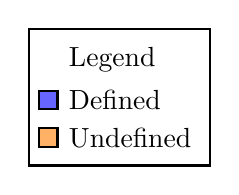
\begin{tikzpicture}
            \matrix [thick, draw=black] {
            \node[label=right:{Legend}] {}; \\
            \node[thick, shape=rectangle, draw=black, fill=blue!60,   label=right:{Defined}](0) {}; \\
            \node[thick, shape=rectangle, draw=black, fill=orange!60, label=right:{Undefined}](1) {}; \\
            };
        \end{tikzpicture}
    \end{subfigure}
    \caption{Breakdown of how many test approaches are undefined.}
    \label{fig:undefPies}
\end{figure*}

\fi

\subsubsection{Stopping Criteria}\label{stop-crit}

Since we cannot continue looking for new approaches indefinitely, we need a
``stopping criteria'' to let us know when we are ``finished'' looking for test
approaches in the literature. Our original plan was to iterate steps
\ref{record-apps} and \ref{record-terms} until there are diminishing returns,
which would imply that we had created something approaching a complete
taxonomy! However, due to time constraints, this is infeasible, so our stopping
point is artificially imposed. Ideally, with more time, we would find
definitions for all terms we uncover, as described in \Cref{undef-terms}.

\ifnotpaper
    In addition to these undefined terms, some terms do not appear in
    the literature at all! While most test approaches arise as a result of our
    snowballing approach, we each have preexisting knowledge of what test
    approaches exist (a form of experience-based testing, if you will).
    As an example, we are surprised that property-based testing is not mentioned
    in any sources investigated, even considering it as a potential stopping point
    during our research%\thesisissueref{57,81,88,125}\qtodo{I think these issue
    % refs, along with some others may actually be worth keeping in our final
    % thesis/paper; thoughts?}
    . Test approaches such as these that arise independently of snowballing
    may serve as starting points for continued research if we do not find
    them in the literature using our iterative approach. The following terms come
    from previous knowledge, conversations with colleagues, research for other
    projects, or ad hoc cursory research to see what other test approaches exist:
    \newline

    \begin{minipage}{\textwidth}
        \begin{multicols}{2}
            \begin{enumerate}
                \item Chaos engineering
                \item Chosen-ciphertext \ifnotpaper\else \\ \fi attacks
                \item Concolic testing
                \item Concurrent testing
                \item Destructive testing
                \item Dogfooding
                \item Implementation-based testing
                \item Interaction-based \ifnotpaper\else \\ \fi testing
                      \ifnotpaper\else\columnbreak\fi
                \item Lunchtime attacks\ifnotpaper%
                          \footnote{In previous meetings, Dr.~Smith mentioned
                              that with the number of test approaches that suggest
                              that people just like to label everything as
                              ``testing'', he would not be surprised if something
                              like ``Monday morning testing'' existed. While
                              independently researching chosen-ciphertext attacks
                              out of curiosity, this prediction of a time-based
                              test approach came true with ``lunchtime attacks''.}
                      \fi
                \item Parallel testing
                \item Property-based testing
                \item Pseudo-random bit \ifnotpaper\else \\ \fi testing
                \item Rubber duck testing
                \item Scream testing
                \item Shadow testing
                \item Situational testing
            \end{enumerate}
        \end{multicols}
    \end{minipage}
\fi
